% arara: closepdf
% arara: xelatex
% arara: showfile
\documentclass{article}
\usepackage[utf8]{inputenc} %probably not needed ...
\usepackage[T1]{fontenc}
\usepackage{fontspec}
\usepackage{marvosym,stmaryrd}
\usepackage{geometry}
\geometry{papersize={128mm,96mm},margin=0.5cm} %\textwidth=11.8, \textheight=8.6
\usepackage[x11names]{xcolor}
\usepackage{tikzducks}
\usetikzlibrary{shapes.geometric, shapes.callouts}
\usetikzlibrary{decorations.text}
\pagestyle{empty}
\parindent=0pt
\usepackage{animate}
\usepackage{eso-pic}
\usepackage{xfp}
\usepackage{ifthen}
\newcommand*{\pineapple}{%
	\begingroup\fontspec{Segoe UI Symbol}\symbol{"1F34D}\endgroup
}
\newcommand{\tovaglia}{([yshift=1cm]partenza) -- ++(4.4em,0) -- ++(1em, -4ex) -- ++(-6.4em,0) -- cycle}
\tikzset{%
	ringhiera/.style = {line width=2pt, green}
} 

\begin{document}
	\AddToShipoutPictureBG{%
		\AtPageLowerLeft{%
			\begin{tikzpicture}[overlay,remember picture]
			\draw[fill=green!10] (0,0) rectangle (\paperwidth,\paperheight);
			\node at (.5\paperwidth,.68\paperheight) {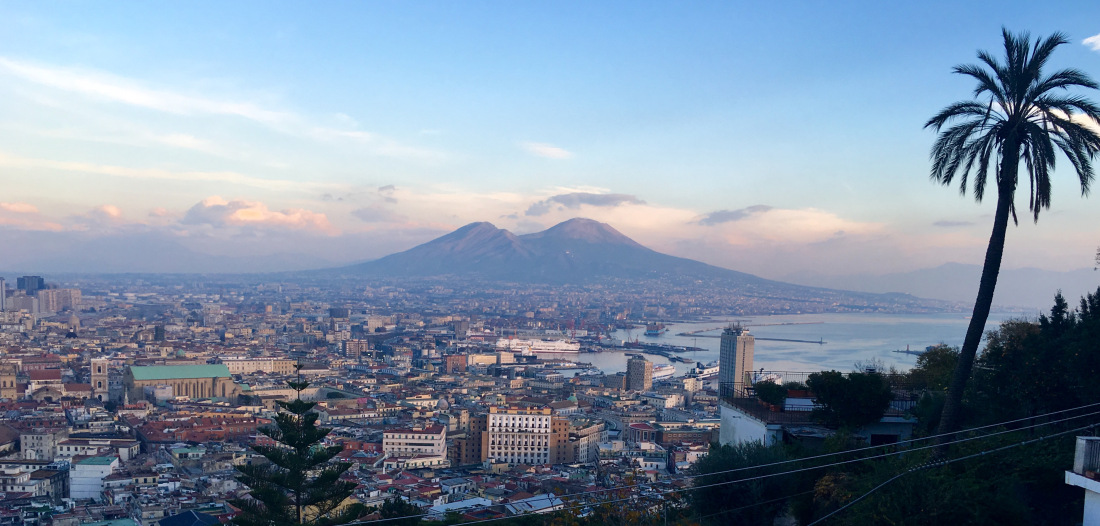
\includegraphics[width=\paperwidth, 
				keepaspectratio]
				{Napoli.jpg}};
			% ringhiera
			\draw[ringhiera] (3,5) -- (\paperwidth,5);
			\draw[line width=2pt, green] (3,4.5) -- (\paperwidth,4.5);
			\foreach \pos in {3,3.5, ..., \paperwidth}{
				\draw[line width=2pt, green] (\pos,4.5) -- (\pos,3);
				\begin{scope}
					\clip (3,3) rectangle (\paperwidth,5);
					\draw[ringhiera] (\pos, 4) circle (1cm);
				\end{scope}
			}
			% casa
			\draw[draw=gray, very thin, fill=yellow!30] (0,3) rectangle (3,\paperheight);
			% porta
			\filldraw[brown] (0.5,3) rectangle +(2,4);
			% insegna
			\node[fill=cyan!30,rectangle, text width=2.2cm, text centered,
				font=\bfseries\itshape,
				draw=blue,
				text=blue] at (1.5,7) {Pizzeria \\ tradizionale};
			\path[postaction={decorate,decoration={text along path,text align=center,text={|\bfseries\color{red}|Da Gennaro}}}] (.5,7.05) arc (180:0:1);
			\end{tikzpicture}}}
		\begin{tikzpicture}
		\path (0,0) rectangle (.99\textwidth, .99\textheight);
		\begin{scope}[xscale=-1, yshift=2ex, transform shape]
		\duck[beard=gray!30, %sunglasses=black, 
			jacket=blue,
			tshirt=cyan,
			book=\scalebox{0.5}{\reflectbox{\TeX}},
			bookcolour=black!20!brown,
			shorthair=gray!30,name=David]
		\end{scope}
		\begin{scope}[xshift=7em, yshift=2ex,]
		\duck[name=waitress, longhair=brown, pizza]
		\end{scope}
		\node[ellipse callout, text=black, draw, fill=white, text width=6.5em, align=center, font=\small,yshift=10ex, xshift=-3em] at (David-head) {A \\ pineapple pizza,\\ please!};
		\node[ellipse callout, text=black, draw, fill=white, text width=7em, align=center, font=\small,yshift=10ex, xshift=-4em] at (waitress-head) {Sorry,\\ we don't have it\\ on the menu!};
		\node[align=center, draw, fill=white, text=red, cloud callout, cloud puffs=15, 
		cloud puff arc=140, callout pointer segments=3,
		inner sep=0pt, anchor=pointer, callout relative pointer={(-.7,-.7)}, aspect=3,yshift=-1ex,font=\bfseries,
		xshift=3.5em] at (waitress-head) {\begin{tabular}{c}
			Wait\dots what?!?! \\ \MVAt $\ \lightning\!\!$ \pineapple $\otimes$ \#
			\end{tabular}};
		\coordinate (partenza) at (0,1.8ex);
		\draw[fill=brown, rounded corners=2] (partenza) rectangle +(.4em,1);
		\draw[fill=brown, rounded corners=2] ([xshift=4em]partenza) rectangle +(.4em,1);
		\path[fill=white] \tovaglia;
		\begin{scope}
		\clip \tovaglia;
		\foreach \y in {-10, 0, ..., 100} {
			\foreach \x in {-10, 0, ..., 100} {
				\path[fill=pink]  ([xshift=5pt]\x pt,\y pt) rectangle +(5pt,5pt);
				\path[fill=pink]  ([yshift=5pt]\x pt,\y pt) rectangle +(5pt,5pt);
				\path[fill=red]  (\x pt,\y pt) rectangle +(5pt,5pt);
			}
		}
		\end{scope}
		\draw \tovaglia; 
	\end{tikzpicture}
\end{document}